\begin{questions}

\fullwidth{
\textbf{\underline{ตอนที่ 1}} จงกากบาทคำตอบที่ถูกต้อง ลงไปในกระดาษคำตอบ \textbf{หน้าที่ \pageref{ans_part_1}} \\
}

\filbreak
  \question ความรู้ทางวิทยาศาสตร์เปลี่ยนแปลง\mbox{หรือไม่}
  \begin{choices}
    \choice ได้ เมื่อมีนักวิทยาศาสตร์ที่เก่งกว่าว่าบอก
    \choice ได้ เมื่อมีเหตุผลหรือหลักฐานที่ดีกว่า
    \choice ไม่ได้ เพราะความรู้ทางวิทยาศาสตร์ได้พิสูจน์แล้ว
    \choice ไม่ได้ เพราะความรู้ทางวิทยาศาสตร์เป็นความจริงที่ยอมรับกันแล้ว
    \choice ไม่ได้ เพราะความรู้ทางวิทยาศาสตร์มีความน่าเชื่อถือ
\end{choices}

\filbreak
  \question การสังเกตของนักวิทยาศาสตร์ทำให้เกิดสิ่งใดเป็นอันดับแรก
  \begin{choices}
    \choice กฎ
    \choice การทดลอง
    \choice ทฤษฎี
    \choice ปัญหา
    \choice สมมติฐาน
\end{choices}

\filbreak
  \question ในขั้นตอนการตรวจสอบสมมติฐาน ถ้าพบว่าผลที่ได้จากการทดลองไม่สอดคล้องกับสมมติฐาน สามารถมีแนวทางปฏิบัติได้หลายประการ ยกเว้นข้อใด
  \begin{choices}
    \choice แก้ไขผลการทดลอง
    \choice แก้ไขสมมติฐานนั้น
    \choice ตั้งปัญหาใหม่
    \choice ทำการทดลองใหม่
    \choice ยกเลิกสมมติฐานนั้น
\end{choices}

\filbreak
  \question ข้อใดเรียงลำดับการทำ Scientific research ได้ถูกต้อง
  \begin{choices}
    \choice Collecting evidence/data - Selecting a topic - Focusing the question
    \choice Designing the study - Interpreting findings - Analyzing findings
    \choice Interpreting findings - Analyzing findings - Designing the study
    \choice Reviewing the literature - Designing the study - Collecting evidence/data
    \choice Selecting a topic - Interpreting findings - Analyzing findings
\end{choices}

\filbreak
  \question ประเภทของข้อมูลทางวิทยาศาสตร์ที่เป็นข้อมูลแบบคุณภาพและปริมาณ เรียกว่าข้อมูลแบบใด (เรียงตามลำดับ)
  \begin{choices}
    \choice Emic \& Etic
    \choice Etic \& Emic
    \choice Qualitative \& Quantitative
    \choice Quantitative \& Qualitative
    \choice Reliability \& Statistics
\end{choices}

\filbreak
  \question นักศึกษาคนหนึ่งต้องการจะศึกษาและวัดระดับความพึงพอใจของผู้ซื้อที่มีต่อคุณภาพสินค้าและผู้ค้าในตลาดนัด แต่นักศึกษากลับทำแบบสอบถามเพื่อไปเก็บข้อมูลความพึงพอใจจากผู้ค้าในตลาดนัด นักศึกษาคนดังกล่าวศึกษาข้อมูลผิดในประเด็นใด
  \begin{choices}
    \choice Hypothesis
    \choice Induction
    \choice Reduction
    \choice Reliability
    \choice Validity
\end{choices}

\filbreak
  \question นักศึกษาคนหนึ่งต้องการจะศึกษาและวัดระดับความพึงพอใจของผู้ซื้อที่มีต่อคุณภาพสินค้าและผู้ค้าในตลาดนัด แต่นักศึกษากลับทำแบบสอบถามเพื่อไปเก็บข้อมูลความพึงพอใจจากผู้ค้าในตลาดนัด ถ้านักศึกษาคนดังกล่าวไปเก็บข้อมูลความพึงพอใจจากผู้ซื้อเพียง 3 คนและนำมาเขียนบทสรุปและนำเสนอ งานวิจัยสำรวจดังกล่าว นักศึกษาคนดังกล่าวศึกษาข้อมูลผิดในประเด็นใด
  \begin{choices}
    \choice Hypothesis
    \choice Induction
    \choice Reduction
    \choice Reliability
    \choice Validity
\end{choices}

\filbreak
  \question ระดับการจัดระเบียบการศึกษาสิ่งมีชีวิตที่เล็กที่สุดในการศึกษาด้านชีววิทยาเรียกว่าอะไร
  \begin{choices}
    \choice Atoms
    \choice Cell
    \choice Molecule
    \choice Organ
    \choice Tissue
\end{choices}

\filbreak
  \question องค์ประกอบที่สำคัญและจำเป็นที่สุดใน Ecosystem คือข้อใด
  \begin{choices}
    \choice แบคทีเรียและพืชสีเขียว
    \choice ผู้ผลิตและผู้บริโภค
    \choice พลังงานแสงและการสังเคราะห์ด้วยแสง
    \choice วัฏจักรของสารและการถ่ายทอดพลังงาน
    \choice ออกซิเจนและคาร์บอนไดออกไซด์
\end{choices}

\filbreak
  \question สภาพของสิ่งแวดล้อมที่ทำให้สิ่งมีชีวิตแสดงพฤติกรรมเรียกว่าอะไร
  \begin{choices}
    \choice Appearance
    \choice Complexity
    \choice Homeostasis
    \choice Reproduction
    \choice Stimuli
\end{choices}

\filbreak
  \question กระบวนการที่นำเอาของเสียออกจากร่างกายของสิ่งมีชีวิตเรียกว่าอะไร
  \begin{choices}
    \choice Excretion
    \choice Movement
    \choice Reproduction
    \choice Respiration
    \choice Sensitivity
\end{choices}

\filbreak
  \question ข้อใดกล่าวถึง Metabolism ได้ไม่ถูกต้อง
  \begin{choices}
    \choice เชลล์อาจได้พลังงานจากกระบวนการ Metabolism
    \choice เป็นกระบวนการที่เกิดเฉพาะในสัตว์
    \choice เป็นการสร้างสารขนาดใหญ่จากสารขนาดเล็ก
    \choice เป็นการสลายสารอาหารเพื่อให้ได้พลังงาน
    \choice เป็นทั้งกระบวนการสร้างและสลายสารชีวโมเลกุล
\end{choices}

\filbreak
  \question สารชีวโมเลกุลชนิดใดที่ทำหน้าที่ให้พลังงานแก่สิ่งมีชีวิตเป็นหลัก
  \begin{choices}
    \choice Carbohydrates
    \choice Lipids
    \choice Nucleic Acids
    \choice Phospholipids
    \choice Proteins
\end{choices}

\filbreak
  \question สารชีวโมเลกุลชนิดใดที่ทำหน้าที่ห่อหุ้มและทำให้เซลล์สัตว์คงรูปร่างได้
  \begin{choices}
    \choice Carbohydrates
    \choice Lipids
    \choice Nucleic Acids
    \choice Nucleotides
    \choice Proteins
\end{choices}

\filbreak
  \question บทบาทที่สำคัญของ Nucleic Acids คืออะไร
  \begin{choices}
    \choice ช่วยในการเจริญเติบโต
    \choice ถ่ายทอดลักษณะทางพันธุกรรม
    \choice ทำให้เกิดโครงสร้างของเซลล์
    \choice เป็นพาหนะพาสารเข้าออกเซลล์
    \choice สลายให้พลังงาน
\end{choices}

\newpage

\fullwidth{
\textbf{\underline{ตอนที่ 2}} จงกากบาทคำตอบที่ถูกต้อง ลงไปในกระดาษคำตอบ \textbf{หน้าที่ \pageref{ans_part_2}} \\
}

\filbreak
  \question สารชีวโมเลกุลชนิดใดที่ทำหน้าที่ช่วยลดพลังงานกระตุ้นเพื่อให้เซลล์มีกิจกรรมทางชีวเคมีที่เหมาะสม
  \begin{choices}
    \choice Carbohydrates
    \choice Enzymes
    \choice Lipids
    \choice Monosaccharides
    \choice Nucleic Acids
\end{choices}

\filbreak
  \question ข้อใดกล่าวถูกต้อง
  \begin{choices}
    \choice เอนไซม์ carbohydrase เกี่ยวข้องกับการเปลี่ยนคาร์โบไฮเดรตเป็นกลูโคส
    \choice เอนไซม์ catalase เกี่ยวข้องกับการเปลี่ยนไฮโดรเจนเปอร์ออกไซด์เป็นน้ำและก๊าซออกซิเจน
    \choice เอนไซม์ lipase เกี่ยวข้องกับการเปลี่ยนไขมันเป็นกลีเซอรอลและกรดไขมัน
    \choice เอนไซม์ protease เกี่ยวข้องกับการเปลี่ยนโปรตีนเป็นกรดอะมิโน
    \choice ถูกทุกข้อ
\end{choices}

\filbreak
  \question ผู้ค้นพบเซลล์เป็นคนแรกคือ
  \begin{choices}
    \choice Antoni Cooke
    \choice Antoni Vancouver
    \choice Antoni van Leeuwenhoek
    \choice Robert Hooke
    \choice Robert van Leeuwencooke
\end{choices}

\filbreak
  \question ทฤษฎีเซลล์มีหลักการอยู่ทั้งหมดกี่ข้อ
  \begin{choices}
    \choice 2
    \choice 3
    \choice 4
    \choice 5
    \choice ไม่มีคำตอบที่ถูกต้อง
\end{choices}

\filbreak
  \question เซลล์ทุกชนิดจะประกอบไปด้วยองค์ประกอบดังต่อไปนี้ ยกเว้น
  \begin{choices}
    \choice Chromosomes
    \choice Cytosol
    \choice Plasma membrane
    \choice Ribosomes
    \choice ไม่มีคำตอบที่ถูกต้อง
\end{choices}

\filbreak
  \question ข้อใดไม่ถูกต้องตามหลักการทางวิทยาศาสตร์ที่เกี่ยวข้องกับ Prokaryotic cell
  \begin{choices}
    \choice เป็นชนิดของเซลล์ของ Domain Bacteria และ Domain Archaea
    \choice เป็นเซลล์ชนิดแรก ๆ ที่ถือกำเนิดบนโลก
    \choice ไม่พบนิวเคลียส
    \choice ไม่พบ nucleolus
    \choice ไม่พบ organelle
\end{choices}

\filbreak
  \question ข้อใดไม่ถูกต้องตามหลักการทางวิทยาศาสตร์ที่เกี่ยวข้องกับ Eukaryotic cell
  \begin{choices}
    \choice เป็นชนิดของเซลล์ของ protists
    \choice พบเยื่อหุ้ม organelles
    \choice พบ organelles
    \choice พบ ribosomes
    \choice ไม่พบ nucleolus
\end{choices}

\filbreak
  \question การมีอยู่ของคุณสมบัติใดที่แยกเซลล์ใน Domain Bacteria ออกจากเซลล์ใน Domain Eukarya
  \begin{choices}
    \choice Cell wall
    \choice DNA
    \choice Flagella
    \choice Membranous organelles
    \choice RNA
\end{choices}

\filbreak
  \question ข้อใดไม่ถูกต้องตามหลักการทางวิทยาศาสตร์ที่เกี่ยวข้องกับ cell wall
  \begin{choices}
    \choice Animal cell wall ประกอบไปด้วย glycogen เป็นหลัก
    \choice Archaea's cell wall ประกอบไปด้วย glycoprotein S-layers เป็นหลัก
    \choice Bacterial cell wall ประกอบไปด้วย peptidoglycan เป็นหลัก
    \choice Fungal cell wall ประกอบไปด้วย chitin เป็นหลัก
    \choice Plant cell wall ประกอบไปด้วย cellulose เป็นหลัก
\end{choices}

\filbreak
  \question ส่วนประกอบของเซลล์ข้อใด ไม่มีเยื่อหุ้ม, มีเยื่อหุ้ม 1 ชั้น และมีเยื่อหุ้ม 2 ชั้น ตามลำดับ
  \begin{choices}
    \choice Lysosome, Mitochondria, Chloroplast
    \choice Mitochondria, Ribosome, Vacuole
    \choice Ribosome, Lysosome, Mitochondria
    \choice Vacuole, Ribosome, Chloroplast
    \choice Vacuole, Ribosome, Mitochondria
\end{choices}

\filbreak
  \question ภายใน single cell ข้อใดต่อไปนี้มีขนาดเล็กที่สุด
  \begin{choices}
    \choice Cell membrane
    \choice Chloroplast
    \choice Mitochondrion
    \choice Nuclear envelope
    \choice Ribosome
\end{choices}

\filbreak
  \question โครงสร้างใดที่ทำหน้าที่สร้าง ribosome
  \begin{choices}
    \choice DNA
    \choice Endoplasmic reticulum
    \choice Golgi apparatus
    \choice Lysosome
    \choice Nucleolus
\end{choices}

\filbreak
  \question rough ER ต่างจาก smooth ER เพราะอะไร
  \begin{choices}
    \choice rough ER ผลิตไขมันเป็นหลัก
    \choice rough ER ผลิตองค์ประกอบของ peroxisome
    \choice rough ER มี ribosome
    \choice rough ER สร้าง transport vesicles
    \choice smooth ER เชื่อมต่อกับ Golgi apparatus
\end{choices}

\filbreak
  \question โครงสร้างใดมีหน้าที่หลักในการรักษารูปร่างของเซลล์โดยเฉพาะในเซลล์สัตว์
  \begin{choices}
    \choice cell wall
    \choice cytosol
    \choice Intermediate filaments
    \choice microfilaments
    \choice microtubules
\end{choices}

\filbreak
  \question ข้อใดกล่าวไม่ถูกต้องเกี่ยวกับ Centriole
  \begin{choices}
    \choice เป็น Organelle ที่ไม่สามารถจำลองตัวเองได้
    \choice พบได้ที่ Centrosome
    \choice มีหน้าที่เกี่ยวข้องกับกระบวนการแบ่งเซลล์
    \choice มี Microtubule เป็นองค์ประกอบหลัก
    \choice ไม่มีคำตอบที่ถูกต้อง
\end{choices}

\filbreak
  \question Organelle ที่มีส่วนประกอบภายในโครงร่างเป็น 9+2 คือข้อใด
  \begin{choices}
    \choice Basal Body
    \choice Centriole
    \choice Chloroplast
    \choice Flagellum
    \choice Lysosome
\end{choices}

\filbreak
  \question Organelle ที่มีส่วนประกอบภายใน โครงร่างเป็น 9+0 คือข้อใด
  \begin{choices}
    \choice Basal Body
    \choice Chloroplast
    \choice Cilia
    \choice Flagellum
    \choice Lysosome
\end{choices}

\filbreak
  \question organelles ใดมีบทบาทที่สำคัญมากที่สุดในการแบ่งเซลล์
  \begin{choices}
    \choice Centrioles
    \choice Endoplasmic Reticulum
    \choice Golgi Apparatus
    \choice Mitochondria
    \choice Peroxisome
\end{choices}

\filbreak
  \question โครโมโซม 1 แท่งจะจำลองตัวเองมาเป็นเส้นคู่แต่ละเส้นของโครโมโซมเรียกว่า
  \begin{choices}
    \choice Centromere
    \choice Chromatid
    \choice Chromatin
    \choice Kinetochore
    \choice Mitotic spindle
\end{choices}

\filbreak
  \question ข้อความใดถูกต้องที่สุดตามหลักการทางวิทยาศาสตร์ ณ ปัจจุบัน
  \begin{choices}
    \choice ก่อนการแบ่งเซลล์จะต้องมีการเพิ่มโครโมโซมก่อน
    \choice kinetochores ยึดจับโครโมโซมที่บริเวณ centromere
    \choice sister chromatids ปกติจะติดกันอยู่ที่บริเวณ centromere
    \choice sister chromatids ปกติจะถูกยึดติดกันด้วย cohesin
    \choice ถูกทุกข้อ
\end{choices}

\newpage
\fullwidth{
จงตอบคำถาม ข้อที่ 36-37 จากภาพที่กำหนดดังต่อไปนี้ \\
\begin{center}
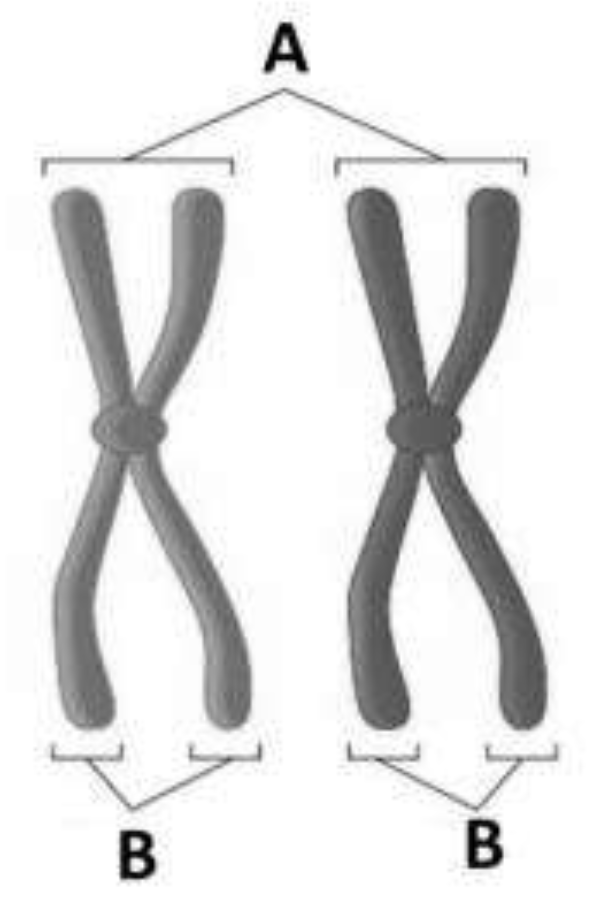
\includegraphics[width=0.4\linewidth]{images/Chromosome.png}
\end{center}
}
\filbreak
  \question ในภาพ “A” คือ
  \begin{choices}
    \choice euchromatin
    \choice heterochromatin
    \choice homologs
    \choice sister chromatids
    \choice synapsis
\end{choices}

\filbreak
  \question ในภาพ “B” คือ
  \begin{choices}
    \choice euchromatin
    \choice heterochromatin
    \choice homologous chromosomes
    \choice homologs
    \choice sister chromatids
\end{choices}

\filbreak
  \question ข้อความใดถูกต้องที่สุดตามหลักการทางวิทยาศาสตร์ ณ ปัจจุบัน
  \begin{choices}
    \choice โปรคาริโอตปกติจะเป็นสิ่งมีชีวิตแบบ haploid
    \choice โปรคาริโอตปกติจะมีโครโมโซมเพียงอันเดียว
    \choice ยูคาริโอตปกติจะเป็นสิ่งมีชีวิตแบบ diploid
    \choice ยูคาริโอตปกติจะมีโครโมโซมมากกว่าหนึ่งอัน
    \choice ถูกทุกข้อ
\end{choices}

\filbreak
  \question เมื่อเปรียบเทียบก่อนและหลังระยะ interphase ของ mitosis ปริมาณใดที่ไม่เพิ่มขึ้นเป็น 2 เท่า
  \begin{choices}
    \choice Centriole
    \choice Centrosome
    \choice Chromatid
    \choice Chromosome
    \choice ถูกทุกข้อ
\end{choices}

\filbreak
  \question เหตุใด checkpoint ที่ควบคุม Cell cycle จึงมีความสำคัญ
  \begin{choices}
    \choice เพราะช่วยป้องกันเซลล์ที่มี DNA เสียหายไม่ให้แบ่งเซลล์
    \choice เพราะเป็นตัวกำหนดว่า DNA ของเชลล์จะถูกคัดลอกได้เร็วแค่ไหน
    \choice เพื่อให้มั่นใจได้ว่า Mitosis เกิดขึ้นต่อเนื่องในทุกเซลล์ของร่างกาย
    \choice เพื่อให้มั่นใจว่า Anaphase จะเกิดหลัง Metaphase เสมอ
    \choice ไม่มีคำตอบที่ถูกต้อง
\end{choices}

\filbreak
  \question การสร้างสายใยสปินเดิลจะเสร็จสิ้นสมบูรณ์ในระยะใดของการแบ่งเซลล์
  \begin{choices}
    \choice ช่วงท้ายของ anaphase
    \choice ช่วงท้ายของ interphase
    \choice ช่วงท้ายของ metaphase
    \choice ช่วงท้ายของ prophase
    \choice ช่วงท้ายของ telophase
\end{choices}

\filbreak
  \question ขณะเซลล์แบ่งตัวแบบ mitosis จะเกิดเส้นใยสปินเดิลขึ้นโดยยึดติดกับส่วนใดในข้อต่อไปนี้
  \begin{choices}
    \choice Centromere
    \choice Chiasmata
    \choice Kinetochore
    \choice Nucleus
    \choice Telomere
\end{choices}

\filbreak
  \question สารที่จำเป็นในการเกิด cytokinesis ในเซลล์สัตว์ คือ
  \begin{choices}
    \choice Actin
    \choice Cyclin
    \choice Microtubule
    \choice Myosin
    \choice Tubulin
\end{choices}

\filbreak
  \question ข้อความใดไม่ถูกต้องตามหลักการทางวิทยาศาสตร์ ณ ปัจจุบัน
  \begin{choices}
    \choice การแบ่งเซลล์แบบไมโตซิสจะได้เซลล์ลูกที่เป็น haploid 2 เชลล์
    \choice การแบ่งเซลล์แบบไมโอซิสจะได้เซลล์ลูกที่เป็น haploid 4 เซลล์
    \choice chiasmata คือบริเวณที่เกิดการแลกเปลี่ยนสารพันธุกรรมระหว่าง homologous chromosome
    \choice Crossing over จะเกิดขึ้นระหว่าง sister chromatids ขณะที่จับคู่กันแบบ synapsis
    \choice ไม่มีคำตอบที่ถูกต้อง
\end{choices}

\filbreak
  \question ข้อใดกล่าวไม่ถูกต้องเกี่ยวกับ crossing over
  \begin{choices}
    \choice เกิดขึ้นในระยะ prophase
    \choice ทุกครั้งที่ต้องการแบ่งเซลล์แบบ meiosis จะต้องเกิด crossing over
    \choice ในเซลล์ที่สร้างขึ้นใหม่มีความหลากหลายของสารพันธุกรรม
    \choice มีการเกิด Chiasma
    \choice มีการแลกเปลี่ยนยืนของ homologous chromosome
\end{choices}

\newpage

\fullwidth{
\textbf{\underline{ตอนที่ 3}} จงกากบาทคำตอบที่ถูกต้อง ลงไปในกระดาษคำตอบ \textbf{หน้าที่ \pageref{ans_part_3}} \\
}

\filbreak
  \question เหตุการณ์ใดจะเกิดขึ้นหลังจากที่แบ่งเซลล์แบบ meiosis I เสร็จสมบูรณ์
  \begin{choices}
    \choice Cytokinesis แบ่ง cytoplasm
    \choice DNA ถูกจำลองเป็นครั้งที่สอง
    \choice Homologous chromosome จะจับคู่กัน
    \choice Homologous chromosome จะแยกออกจากกัน
    \choice ไม่มีคำตอบที่ถูกต้อง
\end{choices}

\filbreak
  \question Chromatids ในเซลล์ของมนุษย์ระยะ Metaphase I มีกี่แท่ง
  \begin{choices}
    \choice 4
    \choice 23
    \choice 46
    \choice 92
    \choice 184
\end{choices}

\filbreak
  \question การแบ่งเซลล์แบบ mitosis แตกต่างจาก meiosis อย่างไร
  \begin{choices}
    \choice mitosis ใช้เวลานานกว่า meiosis
    \choice mitosis ได้เซลล์ที่มีสารพันธุกรรมแตกต่างกัน meiosis ได้เซลล์ที่มีสารพันธุกรรมเหมือนกัน
    \choice mitosis ได้เซลล์ใหม่ 4 เซลล์ meiosis ได้เซลล์ใหม่ 2 เซลล์
    \choice mitosis เป็นการสร้างเซลล์สืบพันธุ์ meiosis สร้างเซลล์ร่างกาย
    \choice mitosis ไม่มีการ Synapsis, Chiasma และ Crossing over
\end{choices}

\filbreak
  \question ข้อใดต่อไปนี้คือตัวอย่างของพลังงานศักย์ในเซลล์สิ่งมีชีวิต
  \begin{choices}
    \choice การเคลื่อนที่ของอะตอม
    \choice การหดตัวของกล้ามเนื้อ
    \choice พลังงานในพันธะเคมีของสารชีวโมเลกุล
    \choice เสียง
    \choice แสง
\end{choices}

\filbreak
  \question ข้อใดจัดเป็นหน้าที่ของ ATP
  \begin{choices}
    \choice เพื่อเปลี่ยนโครงสร้างของโมเลกุลเป้าหมาย
    \choice รับโปรตอนไอออนกลายเป็นน้ำ
    \choice รับอิเล็กตรอนเพื่อส่งต่อให้โปรตีนตัวอื่น
    \choice ให้พลังงานกับโมเลกุลเป้าหมาย
    \choice มีข้อที่ถูกต้องมากกว่า 1 ข้อ
\end{choices}

\filbreak
  \question ข้อใดกล่าวไม่ถูกต้องสำหรับเอนไซม์
  \begin{choices}
    \choice การควบคุมการเกิดเมตาบอลิซึมด้วย negative feedback คือ ผลผลิตที่ได้จะยับยั้งการทำงานของเอนไซม์
    \choice ผลผลิตจะทำหน้าที่เป็นตัวยับยั้งโดยการไปจับที่บริเวณ active site หรือบริเวณอื่น ๆ ของเอนไซม์
    \choice เอนไซม์จะลดพลังงานสุทธิที่ปล่อยออกมา
    \choice เอนไซม์จากมนุษย์ทำงานได้ดีที่อุณหภูมิประมาณ 37 องศาเซลเซียส
    \choice เอนไซม์ทำหน้าที่เร่งปฏิกิริยาเคมี โดยเพิ่มพลังงานกระตุ้นที่ต้องใช้ในปฏิกิริยาเคมี
\end{choices}

\filbreak
  \question ปัจจัยในข้อใดส่งผลต่อกิจกรรมของเอนไซม์
  \begin{choices}
    \choice ความเข้มข้นเกลือ
    \choice ความเข้มข้นของสารตั้งต้น
    \choice อุณหภูมิ
    \choice pH
    \choice ทุกข้อมีผลต่อกิจกรรมของเอนไซม์
\end{choices}

\filbreak
  \question สามารถพบเอนไซม์ได้ที่องค์ประกอบใดของเซลล์ได้บ้าง
  \begin{choices}
    \choice Chloroplast
    \choice Cytosol
    \choice Mitochondria
    \choice Nucleus
    \choice ถูกทุกข้อ
\end{choices}

\filbreak
  \question เอนไซม์ที่ทำหน้าที่สังเคราะห์ ATP มีชื่อว่า
  \begin{choices}
    \choice Amylase
    \choice ATPases
    \choice ATP synthase
    \choice Hydrogen peroxidase
    \choice Oxygenase
\end{choices}

\filbreak
  \question ข้อใดอธิบายการเคลื่อนย้ายสารแบบ simple diffusion ถูกต้อง
  \begin{choices}
    \choice ไม่อาศัยตัวพา ไม่อาศัยพลังงาน เคลื่อนที่ตรงข้าม concentration gradient
    \choice ไม่อาศัยตัวพา ไม่อาศัยพลังงาน เคลื่อนที่ตาม concentration gradient
    \choice ไม่อาศัยตัวพา อาศัยพลังงาน เคลื่อนที่ตาม concentration gradient
    \choice อาศัยตัวพา ไม่อาศัยพลังงาน เคลื่อนที่ตรงข้าม concentration gradient
    \choice อาศัยตัวพา อาศัยพลังงาน เคลื่อนที่ตรงข้าม concentration gradient
\end{choices}

\filbreak
  \question ปัจจัยในข้อใด มีผลต่อทิศทางการแพร่ของอนุภาคของสารผ่านเยื่อเลือกผ่าน
  \begin{choices}
    \choice ขนาดของอนุภาคของสาร
    \choice ความแตกต่างระหว่างความเข้มข้นอนุภาคของสารสองบริเวณ
    \choice ความมีขั้วของสาร
    \choice ชนิดของเยื่อเลือกผ่านที่กั้นอยู่ระหว่างสารทั้งสองสาร
    \choice มีข้อที่ถูกต้องมากกว่า 1 ข้อ
\end{choices}

\filbreak
  \question ข้อใดถูกต้องเกี่ยวกับการเคลื่อนที่ของสารแบบ Facilitated diffusion
  \begin{choices}
    \choice ลำเลียงสารโดยไม่ผ่านเยื่อหุ้มเซลล์
    \choice สารเคลื่อนที่ตรงข้ามกับ concentration gradient
    \choice สารถูกลำเลียงจากบริเวณความเข้มข้นต่ำไปสูง
    \choice อาศัยโปรตีนที่แทรกอยู่ในเยื่อหุ้มเซลล์
    \choice อาศัยพลังงานในรูป ATP
\end{choices}

\filbreak
  \question ข้อใดอธิบายการเคลื่อนย้ายสารผ่านเยื่อเลือกผ่านแบบ active transport ได้ถูกต้อง
  \begin{choices}
    \choice ไม่อาศัยตัวพา ไม่อาศัยพลังงาน เคลื่อนที่ตรงข้าม concentration gradient
    \choice ไม่อาศัยตัวพา ไม่อาศัยพลังงาน เคลื่อนที่ตาม concentration gradient
    \choice ไม่อาศัยตัวพา อาศัยพลังงาน เคลื่อนที่ตาม concentration gradient
    \choice อาศัยตัวพา ไม่อาศัยพลังงาน เคลื่อนที่ตรงข้าม concentration gradient
    \choice อาศัยตัวพา อาศัยพลังงาน เคลื่อนที่ตรงข้าม concentration gradient
\end{choices}

\filbreak
  \question การลำเลียง Na$^+$ และ K$^+$ ผ่านเยื่อหุ้มเซลล์ประสาทขณะถูกกระตุ้น เกิดขึ้นโดยวิธีใด
  \begin{choices}
    \choice Active transport
    \choice Exocytosis
    \choice Facilitated diffusion
    \choice Osmosis
    \choice Simple diffusion
\end{choices}

\filbreak
  \question ข้อใดกล่าวถูกต้องเกี่ยวกับ Endocytosis
  \begin{choices}
    \choice การแพร่ของน้ำเข้าสู่เซลล์
    \choice การลำเลียงสารขนาดใหญ่เข้าสู่เซลล์ด้วย vesicle
    \choice การลำเลียงสารขนาดใหญ่ออกจากเซลล์ด้วย vesicle
    \choice การลำเลียงสารจากบริเวณความเข้มข้นต่ำไปสูง
    \choice การลำเลียงสารไม่มีขั้วและขนาดเล็กผ่านเยื่อหุ้มเซลล์
\end{choices}

\filbreak
  \question กระบวนการ Phagocytosis จัดเป็นกระบวนการประเภทใด
  \begin{choices}
    \choice Active transport
    \choice Endocytosis
    \choice Facilitated diffusion
    \choice Osmosis
    \choice Simple diffusion
\end{choices}

\filbreak
  \question พลังงานแสงอาทิตย์ถูกเปลี่ยนเป็นพลังงานเคมีภายในเซลล์พืชได้โดยกระบวนการใด
  \begin{choices}
    \choice Absorption
    \choice Cellular respiration
    \choice Chemosynthesis
    \choice Oxidation
    \choice Photosynthesis
\end{choices}

\filbreak
  \question กระบวนการสังเคราะห์แสงสามารถใช้พลังงานแสงจากดวงอาทิตย์ในช่วงใด
  \begin{choices}
    \choice Gamma rays
    \choice Infrared
    \choice Ultraviolet
    \choice Visible light
    \choice ถูกทุกข้อ
\end{choices}

\filbreak
  \question หน้าที่ของกระบวนการ light reaction คือการสังเคราะห์สารชนิดใดเพื่อไปใช้ในการ reaction
  \begin{choices}
    \choice ATP และ glucose
    \choice ATP และ NADPH
    \choice ATP และ O$_2$
    \choice Glucose และ O$_2$
    \choice NADPH และ O$_2$
\end{choices}

\filbreak
  \question ข้อใดถูกต้องที่สุดในการอธิบายการสร้าง ATP ในกระบวนการสังเคราะห์แสง ช่วง light reaction
  \begin{choices}
    \choice อาศัยการสร้าง ATP โดยตรงจากระบบแสง 1
    \choice อาศัยการสร้าง ATP โดยตรงจากระบบแสง 2
    \choice อาศัยพลังงานศักย์ที่สะสมใน proton gradient เพื่อสร้าง ATP
    \choice อาศัย NADH ถ่ายทอดอิเล็กตรอน เพื่อสร้าง ATP
    \choice อาศัย NADPH ถ่ายทอดอิเล็กตรอน เพื่อสร้าง ATP
\end{choices}

\filbreak
  \question ผลลัพธ์ทีเกิดจากกระบวนการสังเคราะห์แสง ช่วง dark reaction คือ
  \begin{choices}
    \choice สารอินทรีย์
    \choice สารอินทรีย์ และ ATP
    \choice ATP
    \choice ATP และ NADPH
    \choice NADPH
\end{choices}

\filbreak
  \question ข้อใดกล่าวถูกต้อง
  \begin{choices}
    \choice กระบวนการ light reaction และ dark reaction ในพืช C4 เกิดขึ้นใน bundle sheath cell
    \choice พืชส่วนใหญ่ประมาณ 95\% จัดเป็นพืช C3 เช่น อ้อย ข้าวโพด
    \choice สารอินทรีย์ตัวแรกที่เกิดขึ้นในกระบวนการ dark reaction คือ PGAL
    \choice เอนไซม์ที่ทำหน้าที่ตรึง CO$_2$ ในกระบวนการ dark reaction ชื่อ เอนไซม์ Rubisco
    \choice มีข้อที่ถูกต้องมากกว่า 1 ข้อ
\end{choices}

\filbreak
  \question ข้อใดกล่าวถูกต้องเกี่ยวกับ พืช C3, C4 และ CAM
  \begin{choices}
    \choice C3 และ C4 เปิดปากใบในเวลาที่ต่างกัน คือ กลางวันและกลางคืน ตามลำดับ
    \choice C3 และ C4 มี Calvin cycle เกิดขึ้นในตำแหน่งที่ต่างกัน คือ mesophyll cell และ bundle-sheath cell ตามลำดับ
    \choice C3 และ CAM มี Calvin cycle เกิดขึ้นในตำแหน่งที่ต่างกัน คือ mesophyll cell และ bundle-sheath cell ตามลำดับ
    \choice C3 และ CAM มี Calvin cycle เกิดขึ้นในเวลาต่างกัน คือ กลางวันและกลางคืน ตามลำดับ
    \choice C4 และ CAM มีจำนวนครั้งของการตรึง CO$_2$ ต่างกัน คือ 2 และ 1 ครั้ง ตามลำดับ
\end{choices}

\filbreak
  \question เมื่อร่างกายต้องการพลังงานจากไขมัน ไขมันสามารถถูกย่อยเป็นกลีเซอรอลและกรดไขมัน กลีเซอรอลจะถูกเปลี่ยนไปเป็นสาร intermediate ในขั้น glycolysis ในขณะที่กรดไขมันจะถูกเปลี่ยนไปเป็นสารชนิดใดก่อน
  \begin{choices}
    \choice Acetyl CoA
    \choice ATP
    \choice Citrate
    \choice NADH
    \choice Pyruvate
\end{choices}

\filbreak
  \question กระบวนการ Krebs cycle เกิดขึ้นที่บริเวณใด
  \begin{choices}
    \choice Cytoplasm
    \choice Inner membrane ของ mitochondria
    \choice Intermembrane compartment
    \choice Mitochondria matrix
    \choice Outer membrane ของ mitochondria
\end{choices}

\filbreak
  \question ข้อใดไม่ใช่ผลิตภัณฑ์จากกระบวนการ Krebs cycle
  \begin{choices}
    \choice Acetyl CoA
    \choice ATP
    \choice CO$_2$
    \choice FADH$_2$
    \choice NADH
\end{choices}

\filbreak
  \question โปรตีนที่ทำหน้าที่ในการถ่ายทอดอิเล็กตรอนในกระบวนการหายใจระดับเซลล์ ส่วนใหญ่อยู่ที่บริเวณใด
  \begin{choices}
    \choice ละลายอยู่ในเมทริกซ์
    \choice ละลายอยู่ใน cytosol
    \choice อยู่ที่ช่องระหว่างเยื่อหุ้มชั้นนอกและเยื่อหุ้มชั้นใน
    \choice อยู่ที่เยื่อหุ้มชั้นในของไมโทคอนเดรีย
    \choice อยู่ที่เยื่อหุ้มนอกของไมโทคอนเดรีย
\end{choices}

\filbreak
  \question ในกระบวนการหายใจระดับเซลล์ในสภาวะที่มีก๊าซออกซิเจน ตัวรับอิเล็กตรอนตัวสุดท้ายของ Electron transport chain คือข้อใด
  \begin{choices}
    \choice H$^+$
    \choice H$_2$O
    \choice NAD$^+$
    \choice O$_2$
    \choice pyruvate
\end{choices}

\filbreak
  \question ข้อใดเป็นข้อดีของกระบวนการหมัก (fermentation) เมื่อเปรียบเทียบกับการหายใจระดับเซลล์ที่ใช้ก๊าซออกซิเจน
  \begin{choices}
    \choice ได้คาร์บอนไดออกไซด์
    \choice ได้ปริมาณ ATP เพิ่มขึ้น
    \choice ได้ปริมาณ NADH เพิ่มขึ้น
    \choice ได้ปริมาณ pyruvate เพิ่มขึ้น
    \choice ได้ ATP ในสภาวะที่เซลล์ขาดก๊าซออกซิเจน
\end{choices}

\filbreak
  \question ข้อใดต่อไปนี้กล่าวถูกต้องเกี่ยวกับกระบวนการหมักแอลกอฮอล์
  \begin{choices}
    \choice เกิดการสร้าง ATP จากการถ่ายทอดอิเล็กตรอน
    \choice ได้ NADH เป็นผลิตภัณฑ์
    \choice มีการใช้ก๊าซออกซิเจน
    \choice มีการปลดปล่อยคาร์บอนไดออกไซด์
    \choice pyruvate ถูกเปลี่ยนเป็น methanol
\end{choices}

\end{questions}